%===============================================================================
% $Id: ifacconf.tex 7 2007-11-21 12:50:23Z jpuente $
% Template for IFAC meeting papers
% Copyright (c) 2007 International Federation of Automatic Control
%===============================================================================
\documentclass{ifacconf}
\usepackage[round]{natbib} % you should have natbib.sty
\usepackage{graphicx}      % include this line if your document contains figures

\usepackage{amsmath,amssymb}
\usepackage{url}
\usepackage{diffcoeff}
\usepackage{bm}

\usepackage{mathrsfs}
\usepackage{multirow}

\usepackage{caption, subfig}

\usepackage{xcolor,colortbl}

\newtheorem{remark}{Remark}
\newtheorem{conjecture}{Conjecture}

\DeclareMathOperator*{\argmax}{arg\,max}
\DeclareMathOperator*{\argmin}{arg\,min}
\DeclareMathOperator{\Tr}{Tr}

\def\onedot{$\mathsurround0pt\ldotp$}
\def\cddot{% two dots stacked vertically
	\mathbin{\vcenter{\baselineskip.67ex
			\hbox{\onedot}\hbox{\onedot}}%
}}

\makeatletter \renewcommand\d[1]{\ensuremath{%
		\;\mathrm{d}#1\@ifnextchar\d{\!}{}}}
\makeatother

\bibliographystyle{agsm}
\graphicspath{{./Figures/}}
%===============================================================================
\begin{document}
\begin{frontmatter}

\title{Numerical discretization of port-Hamiltonian plate models \thanksref{footnoteinfo}} 
% Title, preferably not more than 10 words.

\thanks[footnoteinfo]{This work is  supported by the project ANR-16-CE92-0028,
	entitled {\em Interconnected Infinite-Dimensional systems for Heterogeneous
		Media}, INFIDHEM, financed by the French National
	Research Agency (ANR) and the Deutsche Forschungsgemeinschaft (DFG). Further information is available at {\url{https://websites.isae-supaero.fr/infidhem/the-project}}.
	}

\author[ISAE]{Andrea Brugnoli}
\author[ISAE]{Daniel Alazard} 
\author[ISAE]{Val\'erie Pommier-Budinger}
\author[ISAE]{Denis Matignon}

\address[ISAE]{ISAE-SUPAERO, Universit\'e de Toulouse, France.\\
	10 Avenue Edouard Belin, BP-54032, 31055 Toulouse Cedex 4. \\
	Andrea.Brugnoli@isae.fr,  Daniel.Alazard@isae.fr, \\
	Valerie.Budinger@isae.fr, Denis.Matignon@isae.fr}

\begin{abstract}

\end{abstract}

\begin{keyword}
Port-Hamiltonian systems, Kirchhoff Plate, Mindlin-Reissner Plate, Mixed Finite Element Method, Numerical convergence
\end{keyword}

\end{frontmatter}
%===============================================================================

\section{Introduction}


\section{Plate models in port-Hamiltonian form}

In this section the models under consideration are recalled. The details can be found in  \cite{BRUGNOLI2019961,BRUGNOLI2019940}. 

\subsection{Notations}
The space of all, symmetric and skew-symmetric $d\times d$ matrices are denoted by $\mathbb{M}, \mathbb{S}, \mathbb{K}$ respectively. The space of $\mathbb{R}^d$ vectors is denoted by $\mathbb{V}$. $\Omega \subset \mathbb{R}^d$ is an open connected set. The geometric dimension of interest in this paper is $d=2$. For a scalar field $u: \Omega \rightarrow \mathbb{R}$ the gradient is defined as 
\begin{equation*}
\mathrm{grad}(u) =  \nabla u := \begin{pmatrix}
\partial_{x_1} u \dots \partial_{x_d} u \\
\end{pmatrix}^\top.
\end{equation*}
For a vector field $\bm{u}: \Omega \rightarrow \mathbb{V}$, with components $u_j$, the gradient is defined as
\begin{equation*}
\mathrm{grad}(\bm{u})_{i j}:= (\nabla \bm{u})_{ij} = \partial_{x_i} u_j.
\end{equation*}
The symmetric part of the gradient operator $\mathrm{Grad}$ (i. e. the deformation gradient in continuum mechanics) is given by
\begin{equation*}
\mathrm{Grad}(\bm{u}) := \frac{1}{2} \left(\nabla \bm{u} + \nabla^\top \bm{u} \right).
\end{equation*}
The Hessian operator of $u$ is then computed as follows
\begin{equation*}
\mathrm{Hess}(u) = \nabla^2 u = \mathrm{Grad}(\mathrm{grad}(u)),
\end{equation*}
For a tensor field $\bm{U}: \Omega \rightarrow \mathbb{M}$, with components $u_{ij}$, the divergence is a vector, defined column-wise as
\begin{equation*}
\mathrm{Div}(\bm U) = \nabla \cdot \bm{U} := \left( \sum_{i = 1}^d \partial_{x_i} u_{ij} \right)_{j = 1, \dots, d}.
\end{equation*}
The double divergence of a tensor field $\bm{U}$ is then a scalar field defined as
\begin{equation*}
\mathrm{div}(\mathrm{Div}(\bm U)):= \sum_{i, j = 1}^d \partial_{x_i} \partial_{x_j} u_{ij}.
\end{equation*}
The $L^2$ inner products of scalar, vector and matrix field are defined as
\begin{align*}
	(u, v) &= \int_{\Omega} u \ v \d\Omega, \quad u, v : \Omega \rightarrow \mathbb{R}, \\
	(\bm{u}, \bm{v}) &= \int_{\Omega} \bm{u} \cdot \bm{v} \d\Omega, \quad \bm{u}, \bm{v} : \Omega \rightarrow \mathbb{V}, \\
	(\bm{U}, \bm{V}) &= \int_{\Omega} \bm{U} \cddot \bm{V} \d\Omega, \quad \bm{U}, \bm{V} : \Omega \rightarrow \mathbb{M}
\end{align*}
where $\bm{u} \cdot \bm{v} := \sum_{i} u_{i} v_{i}$ is the scalar product in $\mathbb{V}$ and $\bm{U} \cddot \bm{V} := \sum_{i,j} u_{ij} v_{ij}$ is the tensor contraction.
For the tensor field $\bm{U}$, the skew-symmetric part of $\bm{U}$ is $\mathrm{skw}(\bm{U}) = (\bm{U} - \bm{U}^\top)/2$. The standard notation $H^m(\Omega)$ denotes the Sobolev space of $L^2$ integrable functions with  m$^\text{th}$ derivative in $L^2$ and norm $||\cdot||_m$. In particular $H^1_0(\Omega)$ is the space of weakly derivable functions with vanishing trace. For $\mathbb{X} \subseteq \mathbb{M}$, let
\begin{equation*}
\begin{aligned}
H(\mathrm{div}, \Omega) &= \{\bm{u} \in L^2(\Omega, \mathbb{V}) \vert \; \mathrm{div}(\bm{u}) \in L^2(\Omega) \}, \\
H(\mathrm{Div}, \Omega; \mathbb{X}) &= \{\bm{U} \in L^2(\Omega, \mathbb{X}) \vert \; \mathrm{Div}(\bm{U}) \in L^2(\Omega; \mathbb{V}) \},
\end{aligned}
\end{equation*}
which are Hilbert spaces with the norm $||\bm{u}||^2_{\text{div}} = ||\bm{u}||^2 + ||\mathrm{div}(\bm{u})||^2, \; ||\bm{U}||^2_{\text{Div}} = ||\bm{U}||^2 + ||\mathrm{Div}(\bm{U})||^2$. The following abbreviations will be used
\begin{equation*}
\begin{aligned}
M &= H(\mathrm{Div}, \Omega; \mathbb{M}), \\
S &= H(\mathrm{Div}, \Omega; \mathbb{S}),
\end{aligned} \qquad
\begin{aligned}
D &= H(\mathrm{div}, \Omega), \\
L &= L^2(\Omega),
\end{aligned} \qquad
\begin{aligned}
V &= L^2(\Omega; \mathbb{V}), \\
K &= L^2(\Omega; \mathbb{K}).
\end{aligned}
\end{equation*}
Let $\mathcal{X}$ be an Hilbert space $t_f$ a positive real number. We denote by $L^\infty([0, t_f]; \mathcal{X})$ or $L^\infty \mathcal{X}$ the space of functions $f: [0, t_f] \rightarrow X$ for which the time-space norm $||\cdot||_{L^\infty([0, t_f]; \mathcal{X})}$ satisfies
\[
||f||_{L^\infty([0, t_f]; \mathcal{X})} = \mathrm{ess \; sup}_{t \in [0,t_f]} ||f||_{\mathcal{X}} < \infty.
\]


\subsection{Mindlin-Reissner plate}
The Mindlin model is a generalization to the 2D case of the Timoshenko beam model and is expressed by a system of three coupled PDEs (\cite{timoshenko1959theory}) 
\begin{equation}
\begin{cases}
\displaystyle \rho b \diffp[2]{w}{t} &= \mathrm{div}(\bm{q}) + f, \quad (\bm{x}, t) \in \Omega \times [0, t_f]  \vspace{1mm}\\
\displaystyle \frac{\rho b^3}{12} \diffp[2]{\bm \theta}{t} &= \bm{q} + \mathrm{Div}(\bm M) + \bm{\tau}, \\
\end{cases}
\end{equation}
where $\rho$ is the mass density, $b$ the plate thickness, $w$ the vertical displacement, $\bm \theta = (\theta_x, \theta_y)^\top$ collects the deflection of the cross section along axes $x$ and $y$ respectively. The fields $f, \bm{\tau}$ represent distributed forces and momenta. Variables $\bm{M}, \bm{q}$ represent the momenta tensor and the shear stress. The Hooke law relates those to the curvature tensor and shear deformation vector
\begin{equation*}
\begin{aligned}
\bm{M} &:= \mathcal{D} \bm{K} \in \mathbb{S}, \\ \bm{q} &:= \mathcal{C} \bm{\gamma},
\end{aligned} \qquad
\begin{aligned}
\bm{K} &:= \mathrm{Grad}(\bm{\theta}) \in \mathbb{S}, \\ \bm{\gamma} &:= \mathrm{grad}(w) - \bm{\theta}, 
\end{aligned}
\end{equation*}
where $\mathcal{D}, \mathcal{C}$ are symmetric positive tensors
\begin{equation}
\label{eq:bend_rig_tensor}
	\mathcal{D} (\cdot) = \frac{E b^3}{12 (1 - \nu^2)}[(1-\nu)(\cdot) + \nu \Tr(\cdot)], \quad \mathcal{C} (\cdot) = \frac{E b k }{2(1+\nu)}(\cdot),
\end{equation}
where $E$ is the Young modulus, $\nu$ is the Poisson modulus, $k$ is the shear correction factor.
 The kinetic and potential energy  $E_c, E_p$ read
\begin{equation}
\begin{aligned}
E_c &=  \frac{1}{2} \int_{\Omega} \left\{ \rho b \left(\diffp{w}{t} \right)^2 +  \frac{\rho b^3}{12} \diffp{\bm{\theta}}{t} \cdot \diffp{\bm{\theta}}{t}  \right\} \d\Omega, \\
E_p &= \frac{1}{2} \int_{\Omega} \left\{ \bm{M} \cddot \bm{K} + \bm{q} \cdot \bm{\gamma}  \right\}\d\Omega.
\end{aligned}
\end{equation} 
The Hamiltonian  is easily written as $H = E_c + E_p$. To get a port-Hamiltonian formulation suitable energy variables must be selected. The appropriate set is the following
\begin{equation}
\begin{aligned}
\alpha_w &= \rho b \diffp{w}{t}, \\
\bm{A}_{\kappa} &= \bm{K}, \\
\end{aligned} \qquad
\begin{aligned}
\bm\alpha_{\theta} &= \frac{\rho b^3}{12} \diffp{\bm{\theta}}{t}, \\
\bm\alpha_{\gamma} &= \bm{\gamma}. \\
\end{aligned}
\end{equation}
The co-energy variables are found by computing the variational derivative of the Hamiltonian
\begin{equation}
\begin{aligned}
e_w &:= \diffd{H}{\alpha_w} = \diffp{w}{t},  \\
\bm{E}_{\kappa} &:= \diffd{H}{\bm{A}_{\kappa}} = \bm{M}, \\
\end{aligned} \qquad
\begin{aligned}
\bm{e}_{\theta} &:= \diffd{H}{\bm\alpha_{\theta}} = \diffp{\bm{\theta}}{t}, \\
\bm{e}_{\gamma} &:= \diffd{H}{\bm{\alpha}_{\bm{\gamma}}} = \bm{q}. \\
\end{aligned}
\end{equation}
Energy and co-energy are relative by a positive symmetric operator $\bm{\alpha} = \mathcal{H} \bm{e}$
\begin{equation}
\mathcal{H} = \mathrm{diag}(\frac{1}{\rho b}, \; \frac{12}{\rho b^3} , \; \mathcal{D}, \; \mathcal{C})
\end{equation}

The port-Hamiltonian system is expressed as follows 
\begin{equation}
\label{eq:PH_sys_Min_Ten}
\diffp{}{t}
\begin{pmatrix}
\alpha_w \\
\bm\alpha_\theta \\
\bm{A}_\kappa \\
\bm\alpha_{\gamma} \\
\end{pmatrix} = 
\underbrace{\begin{bmatrix}
	0  & 0  & 0  & \mathrm{div} \\
	0 & 0 &  \mathrm{Div} & \bm{I}_{2 \times 2}\\
	0  & \mathrm{Grad}  & 0  & 0\\
	\mathrm{grad} & -\bm{I}_{2 \times 2} &  0 & 0  \\
	\end{bmatrix}}_{\mathcal{J}}
\begin{pmatrix}
e_w \\
\bm{e}_{\theta} \\
\bm{E}_{\kappa} \\
\bm{e}_{\gamma} \\
\end{pmatrix} + 
\begin{pmatrix}
f \\
\bm{\tau} \\
0 \\
0 \\
\end{pmatrix}.
\end{equation}
This system defines a Stokes-Dirac structure, therefore, the boundary values can be found by evaluating the time derivative of the Hamiltonian. In this paper we focus on clamped boundary condition, i.e.
\[
e_w|_{\partial \Omega} = 0, \qquad \bm{e}_{\theta}|_{\partial \Omega} = 0.
\]
More general boundary conditions may be treated as well.

\subsection{Kirchhoff plate}
The Kirchhoff plate model is a generalization to the 2D case of the Euler-Bernoulli beam model. The classical equations for this model are (\cite{timoshenko1959theory}) 
\begin{equation}
\label{eq:clKir}
\displaystyle \rho b \diffp[2]{w}{t} = -\mathrm{div}(\mathrm{Div}(\bm{M})) + f, \quad (\bm{x}, t) \in \Omega \times [0, t_f].
\end{equation}
The bending moment tensor and the curvature are related as in the Mindlin model $\bm{M} = \mathcal{D} \bm{K} \in \mathbb{S}$ (with $\mathcal{D}$ defined in \eqref{eq:bend_rig_tensor}). Following the Kirchhoff assumption the curvature tensor is the Hessian of the vertical displacement
\begin{equation*}
\bm{K} := \mathrm{Grad}(\mathrm{grad}(w)) \in \mathbb{S}.
\end{equation*}
 The kinetic and potential energy $E_c, E_p$ read
\begin{equation}
E_c =  \frac{1}{2}\rho b \left(\diffp{w}{t} \right)^2, \quad
E_p = \frac{1}{2} \bm{M} \cddot \bm{K},
\end{equation} 
The Hamiltonian is then given by $H=E_c + E_p$. Selecting as energy variables
\begin{equation}
\alpha_w = \rho b \diffp{w}{t}, \quad \bm{A}_{\kappa} = \bm{K}, 
\end{equation}
the co-energy variables are found by computing the variational derivative of the Hamiltonian
\begin{equation}
e_w := \diffd{H}{\alpha_w} = \diffp{w}{t}, \quad \bm{E}_{\kappa} := \diffd{H}{\bm{A}_{\kappa}} = \bm{M}, \\
\end{equation}
The coercive operator linking energy and co-energies reads
\begin{equation}
\mathcal{H} = \mathrm{diag}(\frac{1}{\rho b}, \mathcal{D})
\end{equation}
 
The port-Hamiltonian system is expressed as follows 
\begin{equation}
\label{eq:PH_sys_Kir_Ten}
\diffp{}{t}
\begin{pmatrix}
\alpha_w \\
\bm{A}_\kappa \\
\end{pmatrix} = 
\underbrace{\begin{bmatrix}
	0  & -\mathrm{div} \circ \mathrm{Div} \\
	\mathrm{Grad} \circ \mathrm{grad}  & 0 \\
	\end{bmatrix}}_{\mathcal{J}}
\begin{pmatrix}
e_w \\
\bm{E}_{\kappa} \\
\end{pmatrix}+ 
\begin{pmatrix}
f \\
0 \\
\end{pmatrix}.
\end{equation}
Again this system defines a Stokes-Dirac structure and so the boundary values define the power balance. In this paper simply supported boundary conditions are considered, i.e.
\[
e_w|_{\partial \Omega} = 0, \quad \bm{n}^\top \bm{E}_\kappa \bm{n}|_{\partial \Omega}:= m_{\text{nn}}|_{\partial \Omega} = 0.
\]
Differently from the Mindlin plate case, generic boundary conditions demands an accurate analysis, see for instance \cite{Blum1990,mixed_kirchhoff}.

\section{Available mixed finite elements}

In this section suitable semi-discretized are derived for the two models. For the Mindlin plate model two different formulation are presented: the first enforces the symmetry of the momenta tensor strongly, the second weakly. For the Kirchhoff plate, the formulation is based on the the non-conforming Hellan-Herrmann-Johnson method. 

\begin{remark}
System \eqref{eq:PH_sys_Min_Ten}, \eqref{eq:PH_sys_Kir_Ten} can be expressed using either the energy or the co-energy variables. The  most adapted formulation for existing mixed finite element literature is the co-energy based one, which reads
\[
\mathcal{H}^{-1} \partial_t \bm{e} = \mathcal{J} \bm{e}
\]
\end{remark}

\subsection{Mindlin plate with strongly imposed symmetry}

The weak formulation with strongly imposed symmetry seeks $(e_w, \bm{e}_{\bm{\theta}}, \bm{E}_{\kappa}, \bm{e}_{\gamma})$ in $L \times V \times S \times D$ so that 
\begin{equation}
\label{eq:weak_min_PH_strong}
\begin{aligned}
(v_w, \ \rho b \dot{e}_w) &= (v_w, \mathrm{div} \bm{e}_\gamma) + (v_w, f), \\ 
(\bm{v}_\theta, \ \rho b^3/12  \dot{\bm{e}}_\theta) &= (\bm{v}_\theta, \mathrm{Div} \bm{E}_\kappa + \bm{e}_\gamma) + (\bm{v}_\theta, \bm{\tau}), \\  
(\bm{V}_\kappa, \ \mathcal{D}^{-1} \dot{\bm{E}}_\kappa) &= -(\mathrm{Div} \bm{V}_\kappa,  \bm{e}_\theta), \\ 
(\bm{v}_\gamma, \ \mathcal{C}^{-1} \dot{\bm{e}}_\gamma) &= -(\mathrm{div} \bm{v}_\gamma, e_w ) + (\bm{v}_\gamma, \bm{e}_{\theta}), \\ 
\end{aligned} \quad
\begin{aligned}
v_w \in L, \\
\bm{v}_\theta \in V, \\
\bm{V}_\kappa \in S, \\
\bm{v}_\gamma \in D.
\end{aligned}
\end{equation}
This system is obtained by integrating by parts the last two lines of \eqref{eq:PH_sys_Min_Ten} and considering clamped boundary conditions. Obtaining stable finite element that embeds the symmetry of the stress tensor for the general elastodynamics problem has proven to be a difficult task. The easiest implementation manageable by the Firedrake library (\cite{rathgeber2017firedrake}) is the one presented in \cite{becacheWave,becacheElas}. The main disadvantage is that this scheme requires the domain to be given by union of rectangles, as the mesh elements have to be squared. This allows constructing a simple element for the momenta tensor. The polynomial spaces for the discretization are
\[
N_{k} = \{p(x, y)| \; p(x, y) = \sum_{i\le k, j\le k} a_{ij} x^i y^j  \},
\]
Given a regular mesh $\mathcal{Q}_h$ with squared elements $Q$ the following spaces are introduced as discretization spaces
\begin{equation}
\label{eq:BTJ}
	\begin{aligned}
	L_h^{\text{BJT}} &= \{w_h \in L | \ \forall Q, \ w_h|_{Q} \in N_k \}, \\
	V_h^{\text{BJT}} &= \{\bm{\theta}_h \in V | \ \forall Q,\ \bm{\theta}_h|_{Q} \in (N_k)^2 \}, \\
	S_h^{\text{BJT}} &= \{m_{12} \in H^1(\Omega)| \ \forall Q,\ m_{12}|_{Q} \in N_{k+1} \}  \\
	&\cup \{(m_{11}, m_{22}) \in D| \; \forall Q,\ (m_{11}, m_{22})|_{Q} \in N_{k+1} \}, \\
	D_h^{\text{BJT}} &= \{\bm{q}_h \in D | \ \forall Q,\ \bm{q}_h|_{Q} \in N_{k+1} \}, \\ 
	\end{aligned}
\end{equation}
where $BTJ$ stands for the initials of the authors in \cite{becacheWave,becacheElas}.
Combining the results of both papers, the following error estimates are conjectured:
\begin{conjecture}
Assuming a smooth solution to problem \eqref{eq:weak_min_PH_strong}, the following error estimates hold 
\begin{equation}
\label{eq:errBEC}
\begin{aligned}
||e_w - e_w^h||_{L^{\infty} L^2} &\lesssim h^{k+1}, \\
||\bm{e}_\theta - \bm{e}_\theta^h||_{L^{\infty} L^2} &\lesssim h^{k+1}, \\
\end{aligned} \quad
\begin{aligned}
||\bm{E}_\kappa - \bm{E}_\kappa^h||_{L^{\infty} L^2} &\lesssim  h^{k+1}, \\
||\bm{e}_\gamma - \bm{e}_\gamma^ h||_{L^{\infty} L^2} &\lesssim  h^{k+1}, \\
\end{aligned} 
\end{equation}
where the notation $A \lesssim B$ means $A \le C B$. The constant depends only on the true solution and on the final time.
\end{conjecture}


\subsection{Mindlin plate with weakly imposed symmetry}
The formulation \eqref{eq:weak_min_PH_strong} has to be modifies to impose the symmetry of the momenta tensor weakly. Taking the weak form of the third equation in \eqref{eq:PH_sys_Min_Ten}
\[
(\bm{V}_\kappa, \ \mathcal{D}^{-1} \dot{\bm{E}}_\kappa) = (\bm{V}_\kappa, \mathrm{Grad}\bm{e}_\theta ). 
\]
The symmetric gradient can be rewritten as 
\[
\mathrm{Grad}\ \bm{\theta} = \mathrm{grad}\ \bm{\theta} - \mathrm{skw}\mathrm{grad}\ \bm{\theta},
\]
where $\mathrm{skw}(\bm{A})$ is the skew-symmetric part of matrix $\bm{A}$. Introducing the new variable $\bm{E}_r = \mathrm{skw}(\mathrm{grad}(\bm{\theta}))$ then $(\bm{e}_\theta, \bm{E}_\kappa, \bm{E}_r) \in V\times M\times K$ satisfy (reminding that $\bm{e}_\theta = \dot{\bm{\theta}}$)
\begin{equation*}
	\begin{aligned}
	(\bm{V}_\kappa, \ \mathcal{D}^{-1} \dot{\bm{E}}_\kappa) &= (\bm{V}_\kappa, \mathrm{grad}(\bm{e}_\theta)) - (\bm{V}_\kappa, \ \dot{\bm{E}}_r), \\
	&= -(\mathrm{Div}\bm{V}_\kappa, \bm{e}_\theta) - (\bm{V}_\kappa, \ \dot{\bm{E}}_r).
	\end{aligned}
\end{equation*}
The momenta tensor is weakly symmetric if $\bm{V}_r, \ \bm{E}_{\kappa}$. The weak formulation then consists in finding $(e_w, \bm{e}_{\bm{\theta}}, \bm{E}_{\kappa}, \bm{e}_{\gamma}, \bm{E}_{r})$ in $L \times V \times M \times D \times K$ so that 
 \begin{equation}
 \label{eq:weak_min_PH_weak}
 \begin{aligned}
 (v_w, \ \rho b \dot{e}_w) &= (v_w, \mathrm{div} \bm{e}_\gamma) + (v_w, f), \\ 
 (\bm{v}_\theta, \ \rho b^3/12  \dot{\bm{e}}_\theta) &= (\bm{v}_\theta, \mathrm{Div} \bm{E}_\kappa + \bm{e}_\gamma) + (\bm{v}_\theta, \bm{\tau}), \\  
 (\bm{V}_\kappa, \ \mathcal{D}^{-1} \dot{\bm{E}}_\kappa) &= -(\mathrm{Div} \bm{V}_\kappa,  \bm{e}_\theta) - (\bm{V}_\kappa, \ \dot{\bm{E}}_r), \\ 
 (\bm{v}_\gamma, \ \mathcal{C}^{-1} \dot{\bm{e}}_\gamma) &= -(\mathrm{div} \bm{v}_\gamma, e_w ) + (\bm{v}_\gamma, \bm{e}_{\theta}), \\ 
 (\bm{V}_r, \ \dot{\bm{E}}_\kappa) &= 0
 \end{aligned} \quad
 \begin{aligned}
 v_w \in L, \\
 \bm{v}_\theta \in V, \\
 \bm{V}_\kappa \in S, \\
 \bm{v}_\gamma \in D, \\
 \bm{V}_r \in K, \\
 \end{aligned}
 \end{equation}
Consider a regular triangulation $\mathcal{T}_h$ with elements $T$. The space of polynomials of order $k$ on a mesh cell is denoted by $P_k$. The following space are used as discretization spaces

\begin{equation}
\label{eq:AFW}
\begin{aligned}
L_h^{\text{AFW}} &= \{w_h \in L | \ \forall T, \ w_h|_{T} \in P_k \}, \\
V_h^{\text{AFW}} &= \{\bm{\theta}_h \in V | \ \forall T,\ \bm{\theta}_h|_{T} \in (P_k)^2 \}, \\
S_h^{\text{AFW}} &= \{(m_{11}, m_{12}) \in D| \ \forall T,\ (m_{11}, m_{12})|_{T} \in BDM_{[k+1]} \}  \\
& \cup \{(m_{21}, m_{22}) \in D| \ \forall T,\ (m_{21}, m_{22})|_{T} \in BDM_{[k+1]} \}, \\
D_h^{\text{AFW}} &= \{\bm{q}_h \in D | \ \forall T,\ \bm{q}_h|_{T} \in RT_{[k]} \}, \\
K_h^{\text{AFW}} &= \{\bm{R}_h \in K | \ \forall T, \ w_h|_{T} \in P_{[k]} \}, \\ 
\end{aligned}
\end{equation}
where $BDM$ is the Brezzi-Douglas-Marini element and $RT$ the Raviart-Thomas element. The acronym AFW stands for Arnold-Falk-Winther. A convergence analysis for the general elastodynamics problem with weak symmetry is detailed \cite{ArnoldWeak}. A convergence study for the wave equation with mixed finite elements is presented in \cite{Geveci}. Combining the result of the two the following error estimate are conjectured:
\begin{conjecture}
	Assuming a smooth solution to problem \eqref{eq:weak_min_PH_strong}, the following error estimates hold 
	\begin{equation}
	\label{eq:errAFW}
	\begin{aligned}
	||e_w - e_w^h||_{L^{\infty} L^2} &\lesssim h^{k+1}, \\
	||\bm{e}_\theta - \bm{e}_\theta^h||_{L^{\infty} L^2} &\lesssim h^{k+1}, \\
	||\bm{E}_r - \bm{E}_r^h||_{L^{\infty} L^2} &\lesssim h^{k+1}. \\
	\end{aligned} \quad
	\begin{aligned}
	||\bm{E}_\kappa - \bm{E}_\kappa^h||_{L^{\infty} L^2} &\lesssim  h^{k+1}, \\
	||\bm{e}_\gamma - \bm{e}_\gamma^ h||_{L^{\infty} L^2} &\lesssim  h^{k+1}, \\
	\end{aligned} 
	\end{equation}
\end{conjecture}

\subsection{The HHJ scheme for the Kirchhoff plate}
For the Kirchhoff plate, the HHJ scheme can be used to obtain a structure preserving discretization. The discussion follows \cite{arnold2019hellan}. Given the non conforming nature of this scheme, it is necessary to first introduce the discrete functional spaces and state the problem directly in discrete form. The vertical displacement is approximated using continuous Lagrange polynomials, while the momenta tensor is discretized using the HHJ element
\begin{equation}
\label{eq:HHJ}
\begin{aligned}
W_h = &\{w_h \in H^1_0(\Omega)| \; \forall T, \; w_h|_{T} \in P_{k+1} \}, \\
U_h = &\{\bm{M}_h \in L^2(\Omega, \mathbb{S})| \; \forall T, \; \bm{M}_h|_{T} \in P_{k}(\mathbb{S}) , \\ 
&\, \ \bm{M}_h \text{ is normal-normal continuos across elements}\}.
\end{aligned}
\end{equation}
The normal to normal continuous means that if two triangles $T_1, T_2$ share a common edge then $\bm{n}^\top (\bm{M}_h|_{T_1}) \bm{n} = \bm{n}^\top (\bm{M}_h|_{T_2}) \bm{n}$. Taking system \eqref{eq:PH_sys_Kir_Ten} and multiplying the first equation by $v_w \in W_h$ and integrating over a triangle
\begin{equation*}
	\begin{aligned}
	& - (v_w, \ \mathrm{div}\mathrm{Div} \bm{E}_\kappa))_{T} = (\nabla v_w, \ \mathrm{Div} \bm{E}_\kappa))_{T}=, \\
	& -(\nabla^2 v_w, \ \bm{E}_\kappa)_T + (\partial_n v_w, \bm{n}^\top\bm{E}_\kappa \bm{n})_{\partial T} + (\partial_s v_w, \bm{s}^\top\bm{E}_\kappa \bm{n})_{\partial T}. \\
	\end{aligned}
\end{equation*}
A double integration by parts is applied to get the final equation. Summing up over all triangles provides for the penultimate term
\begin{equation*}
\sum_{T \in \mathcal{T}_h} (\partial_n v_w, \bm{n}^\top\bm{E}_\kappa \bm{n})_{\partial T} = \sum_{E \in \mathcal{E}_h} ([\![\partial_n v_w]\!], m_{\text{nn}})_{E},
\end{equation*} 
where $[\![a]\!] = a|_{T_1} + a|_{T_2}$ denotes the jump of a function across share edges. For a boundary edge it is symply the value of the function. For the final term, it holds $(\partial_s v_w, \bm{s}^\top\bm{E}_\kappa \bm{n})_{\partial T}=0$, as $v_w$ is continuous across the edge boundaries and the normal switches sign. We are now in the position to state the final weak form. Given the definition
\[
b_h(v_w, \ \bm{E}_{\kappa}) := - \sum_{T \in \mathcal{T}_h} ( \nabla^2 v_w, \ \bm{E}_\kappa) + \sum_{E \in \mathcal{E}_h} ([\![\partial_n v_w]\!], m_{\text{nn}})_{E}, 
\]
find $(e_w, \bm{E}_\kappa) \in W_h \times U_h$ such that
\begin{equation}
\label{eq:weak_kir_PH}
\begin{aligned}
(v_w, \ \rho b \dot{e}_w) &= +b_h(v_w, \ \bm{E}_{\kappa}) + (v_w, f), \\ 
(\bm{V}_\kappa, \ \mathcal{D}^{-1} \dot{\bm{E}}_\kappa) &= -b_h(e_w, \ \bm{V}_{\kappa}), \\ 
\end{aligned} \quad
\begin{aligned}
v_w \in W_h, \\
\bm{V}_\kappa \in U_h. \\
\end{aligned}
\end{equation}

For the associated static problem, under the hypothesis of smooth solutions optimal convergence of the order $O(k+1)$ for $w \in H^1$ and $\bm{M} \in L^2$ has been established. So, it is natural to conjecture the following result for the dynamic problem:
\begin{conjecture}
Assuming a smooth solution for problem \eqref{eq:weak_kir_PH}, the following error estimates hold
\begin{equation}
\label{eq:errHHJ}
||e_w - e_w^h||_{L^{\infty} H^1} \lesssim h^{k+1}, \qquad
||\bm{E}_\kappa - \bm{E}_\kappa^h||_{L^{\infty} L^2} \lesssim h^{k+1}.
\end{equation}
\end{conjecture}


\section{Numerical experiments}
In this section numerical test cases are used to verify the conjectured orders of convergence for the two problems. Upon discretization, system \eqref{eq:weak_min_PH_strong}, \eqref{eq:weak_min_PH_weak}, \eqref{eq:weak_kir_PH} assumes the from 
\[
M \dot{\bm{e}} = J \bm{e}.
\]
Matrix $J$ is skew symmetric, matrix $M$ is symmetric and positive definite for \eqref{eq:weak_min_PH_strong}, \eqref{eq:weak_kir_PH} while it is symmetric and indefinite for \eqref{eq:weak_min_PH_weak}, because of the multiplier that enforces the symmetry. The Firedrake library \cite{rathgeber2017firedrake} is used to generate the matrices. To integrate the equations in time a Crank-Nicholson scheme has been used, for all simulation. The time step is set to $\Delta t = h/10$ to have a lower impact of the time discretization error when the finite element order is higher than two. The final time is set to one $t_f = 1 [\textrm{s}]$ for all simulations. To compute the $L^\infty \mathcal{X}$ space-time dependent norm  the following approximation is used
\[
||\cdot ||_{L^\infty \mathcal{X}}
\]

\subsection{Numerical test for the Mindlin plate}
Constructing an analytical solution for a vibrating Mindlin plate is not trivial. Therefore, the solution for the static case presented in \cite{mindlinVeiga} is exploited. Consider a distributed static force given by 
\begin{equation*}
\begin{aligned}
f_s(x,y)=\frac{E}{12 (1-\nu^2)} \{12 y(y-1)(5x^2-5x+1)\\
\times [2y^2(y-1)2+x(x-1)(5y^2-5y+1)] +12x(x-1)\\
\times (5y^2-5y+1)[2x^2(x-1)2+y(y-1)(5x^2-5x+1)]\}.
\end{aligned}
\end{equation*}
The static displacement and rotation are given by
\begin{align*}
	w_s(x,y) &= \frac{1}{3} x^3(x-1)^3 y^3 (y-1)^3\\
	&-\frac{2 b^2}{5(1-\nu)}[y^3(y-1)^3 x(x-1)(5 x^2-5x+1). \\
	\bm{\theta}_{s}(x,y) &= 
	\begin{pmatrix}
	y^3(y-1)^3 \ x^2 (x-1)^2 (2x-1) \\
	x^3(x-1)^3 \ y^2 (y-1)^2 (2y-1) \\
	\end{pmatrix}
\end{align*}
The static solution solves the following problem defined on the squared domain $\Omega=(0,1)\times(0,1)$:
\begin{equation}
\begin{aligned}
0 &= \mathrm{div} \ \bm{q}_s + f_s , \\
0 &= \mathrm{Div} \bm{M}_s + \bm{q}_s, \\
\mathcal{D}^{-1} \bm{M}_s &= \mathrm{Grad} \ \bm{\theta}_s, \\
\mathcal{C}^{-1} \bm{q}_s &= \mathrm{grad} \ w_s - \bm{\theta}_s. \\
\end{aligned}
\end{equation}
Given the linear nature of the system a solution for the dynamic problem is found by multiplying the static solution by a time dependent term. For simplicity a sinus function is chosen
\[
w_d(x,y,t) = w_s(x,y) \sin(t), \quad \bm{\theta}_d(x,y,t) = \bm\theta_s(x,y) \sin(t).
\]
For the port-Hamiltonian system velocities are needed
\[
e_w^\text{ex}(x,y,t) = w_s(x,y) \cos(t), \quad \bm{e}_\theta^\text{ex}(x,y,t) = \bm\theta_s(x,y) \cos(t).
\]
The momenta and shear force are then defined by
\[
\bm{M}_d = \bm{E}_\kappa^\text{ex} =  \mathcal{D} \ \mathrm{Grad} \ \bm{\theta}_d, \quad \bm{q}_d = \bm{e}_\gamma^\text{ex} = \mathcal{C}(\mathrm{grad} \ w_d - \bm{\theta}_d)
\]
Appropriate forcing terms have to be introduced. The force and torque in the dynamical case become
\begin{equation*}
f_d = f_s \sin(t) + \rho b \partial_{tt} w_d, \qquad
\bm{\tau}_d = \frac{\rho b^3}{12} \partial_{tt} \bm{\theta}_d
\end{equation*}
Variables $(e_w^\text{ex}, \bm{e}_\theta^\text{ex}, \bm{E}_\kappa^\text{ex}, \bm{e}_\gamma^\text{ex})$ under solicitations $(f_d, \bm{\tau}_d)$ solve problem \eqref{eq:PH_sys_Min_Ten}. The solution being smooth, the conjectured error estimates should hold. The numerical values of the physical parameters are reported in Table \ref{tab:parMin}.

\begin{table}[h]
	\centering
	\begin{tabular}{ccccc}
		\hline 
		\multicolumn{5}{c}{Plate parameters} \\ 
		\hline 
		$E$ & $\rho$ & $\nu$ & $k$ & $h$ \\
		1 $[\textrm{Pa}]$ & $1\; [\textrm{kg}/\textrm{m}^3]$ & 0.3 & 5/6 & 0.1 $[\textrm{m}]$\\ 
		\hline 
	\end{tabular} 
	\captionsetup{width=0.95\linewidth}
	\vspace{1mm}
	\captionof{table}{Physical parameters for the Mindlin plate.}
	\label{tab:parMin}
\end{table}

\paragraph{Results for the strong symmetry formulation} 

The weak form \eqref{eq:weak_min_PH_strong} and its corresponding element \eqref{eq:BTJ} was implemented using Firedrake extruded mesh functionality (\cite{firedrake_extruded}). A direct LU solver based on a LU preconditioner is used. In Fig. \ref{fig:errorBEC} the errors for $(e_w, \bm{e}_\theta, \bm{E}_\kappa, \bm{e}_\gamma)$ are reported. As on one can notice, the conjectured error estimates \eqref{eq:errBEC} are respected for all variables. 

\begin{figure}[ht]%
	\centering
	\subfloat[][$L^\infty L^2$ error for $e_w$]{%
		\label{fig:errBEC1}%
		\includegraphics[width=0.48\columnwidth]{Mindlin/CCCC_BEC__vel.eps}}%
	\hspace{8pt}%
	\subfloat[][$L^\infty L^2$ error for $\bm{e}_\theta$]{%
		\label{fig:errBEC2}%
		\includegraphics[width=0.48\columnwidth]{Mindlin/CCCC_BEC__om.eps}} \\
	\subfloat[][$L^\infty L^2$ error for $\bm{E}_\kappa$]{%
		\label{fig:errBEC3}%
		\includegraphics[width=0.48\columnwidth]{Mindlin/CCCC_BEC__sig.eps}}%
	\hspace{8pt}%
	\subfloat[][$L^\infty L^2$ error for $\bm{e}_\gamma$]{%
		\label{fig:errBEC4}%
		\includegraphics[width=0.48\columnwidth]{Mindlin/CCCC_BEC__q.eps}}%
	\caption[errorBEC]{Error for the Mindlin plate using the BJT element}%
	\label{fig:errorBEC}%
\end{figure}

\paragraph{Results for the weak symmetry formulation} 
Formulation \eqref{eq:weak_min_PH_weak} and its element \eqref{eq:AFW} are here considered. A direct LU solver failed for high order cases (i.e. $k=3$). For this reason a generalized minimal residual method is used with restart number of iterations equal to 100. In Fig. \ref{fig:errorAFW} the errors for $(e_w, \bm{e}_\theta, \bm{E}_\kappa, \bm{e}_\gamma, \bm{E}_r)$ different variables are reported. The errors for $(e_w, \bm{e}_\theta, \bm{e}_\gamma)$ respect the conjecture result \eqref{eq:errAFW}. Variables $(\bm{E}_\kappa, \bm{E}_r)$ exhibit a superconvergence phenomenon for the case $k=1$. Furthermore, the convergence order of $(\bm{E}_\kappa, \bm{e}_\gamma, \bm{E}_r)$ deteriorates for $k=3$ for the finest mesh. This must be linked to reduced integration errors or to the time discretization error that may overcome the spatial discretization error. Indeed in \cite{ArnoldWeak} an hybridization method is used to solve the elastodynamics problem in time. This avoids the need for solving a saddle-point problem.

\begin{figure}[ht]%
	\centering
	\subfloat[][$L^\infty L^2$ error for $e_w$]{%
		\label{fig:errAFW1}%
		\includegraphics[width=0.48\columnwidth]{Mindlin/CCCC__vel.eps}}%
	\hspace{8pt}%
	\subfloat[][$L^\infty L^2$ error for $\bm{e}_\theta$]{%
		\label{fig:errAFW2}%
		\includegraphics[width=0.48\columnwidth]{Mindlin/CCCC__om.eps}} \\
	\subfloat[][$L^\infty L^2$ error for $\bm{E}_\kappa$]{%
		\label{fig:errAFW3}%
		\includegraphics[width=0.48\columnwidth]{Mindlin/CCCC__sig.eps}}%
	\hspace{8pt}%
	\subfloat[][$L^\infty L^2$ error for $\bm{e}_\gamma$]{%
		\label{fig:errAFW4}%
		\includegraphics[width=0.48\columnwidth]{Mindlin/CCCC__q.eps}}%
	\subfloat[][$L^\infty L^2$ error for $\bm{E}_r$]{%
	\label{fig:errAFW5}%
	\includegraphics[width=0.48\columnwidth]{Mindlin/CCCC__r.eps}}%
	\caption[errorAFW]{Error for the Mindlin plate using the AFW element}%
	\label{fig:errorAFW}%
\end{figure}

 
\subsection{Numerical test for the Kirchhoff plate}
An analytical solution for the Kirchhoff plate is readily available (see for instance \cite{reddy2006theory}). Consider the following solution of problem \eqref{eq:clKir} under simply supported conditions on a squared unitary domain
\[
w^{\text{ex}}(x,y,t) = \sin(\pi x) \sin(\pi y) \sin(t), \quad  (x, y) \in (0,1)\times (0,1).
\] 
The corresponding forcing term is given by 
\[
f = (4 D \pi^4 - \rho b) \sin(\pi x) \sin(\pi y) \sin(t), \quad D = \frac{E b^3}{12 (1-\nu^2)}.
\]
The corresponding variables in the port-Hamiltonian frame work are
\[
e_w^{\text{ex}} = \partial_t w^{\text{ex}}, \quad \bm{E}_\kappa^{\text{ex}} = \mathcal{D} \nabla^2 w^{\text{ex}}
\]
Variables $(e_w^{\text{ex}}, \bm{E}_\kappa^{\text{ex}})$ under solicitation $f$ solve problem \eqref{eq:PH_sys_Kir_Ten}. The physical parameters used in simulation are reported in Table \ref{tab:parKir}. \\
The weak form \eqref{eq:weak_kir_PH} and the element \eqref{eq:HHJ} are now considered.
A direct solver with LU preconditioner is used to compute the solution. Results are shown in Fig. \ref{fig:errorHHJ}. The conjectured error estimates
\begin{table}[h]
	\centering
	\begin{tabular}{cccc}
		\hline 
		\multicolumn{4}{c}{Plate parameters} \\ 
		\hline 
		$E$ & $\rho$ & $\nu$  & $h$ \\
		136 $[\textrm{GPa}]$ & $5600\; [\textrm{kg}/\textrm{m}^3]$ & 0.3 &  0.001 $[\textrm{m}]$\\ 
		\hline 
	\end{tabular} 
	\captionsetup{width=0.95\linewidth}
	\vspace{1mm}
	\captionof{table}{Physical parameters for the Kirchhoff plate.}
	\label{tab:parKir}
\end{table}

\begin{figure}[ht]%
	\centering
	\subfloat[][$L^\infty H^1$ error for $e_w$]{%
		\label{fig:errHHJ1}%
		\includegraphics[width=0.48\columnwidth]{Kirchhoff/SSSS__vel.eps}}%
	\hspace{8pt}%
	\subfloat[][$L^\infty L^2$ error for $\bm{E}_\kappa$]{%
		\label{fig:errHHJ2}%
		\includegraphics[width=0.48\columnwidth]{Kirchhoff/SSSS__sig.eps}} \\
	\caption[errorHHF]{Error for the Kirchhoff plate using the HHJ element}%
	\label{fig:errorHHJ}%
\end{figure}


\begin{ack}
The authors would like to thank Michel Sala\"un from ISAE-SUPAERO for the fruitful and insightful discussions.
\end{ack}

\bibliography{biblio_MTNS}             % bib file to produce the bibliography
                                                     % with bibtex (preferred)
                                                   
%\begin{thebibliography}{xx}  % you can also add the bibliography by hand

%\bibitem[Able(1956)]{Abl:56}
%B.C. Able.
%\newblock Nucleic acid content of microscope.
%\newblock \emph{Nature}, 135:\penalty0 7--9, 1956.

%\bibitem[Able et~al.(1954)Able, Tagg, and Rush]{AbTaRu:54}
%B.C. Able, R.A. Tagg, and M.~Rush.
%\newblock Enzyme-catalyzed cellular transanimations.
%\newblock In A.F. Round, editor, \emph{Advances in Enzymology}, volume~2, pages
%  125--247. Academic Press, New York, 3rd edition, 1954.

%\bibitem[Keohane(1958)]{Keo:58}
%R.~Keohane.
%\newblock \emph{Power and Interdependence: World Politics in Transitions}.
%\newblock Little, Brown \& Co., Boston, 1958.

%\bibitem[Powers(1985)]{Pow:85}
%T.~Powers.
%\newblock Is there a way out?
%\newblock \emph{Harpers}, pages 35--47, June 1985.

%\bibitem[Soukhanov(1992)]{Heritage:92}
%A.~H. Soukhanov, editor.
%\newblock \emph{{The American Heritage. Dictionary of the American Language}}.
%\newblock Houghton Mifflin Company, 1992.

%\end{thebibliography}

\appendix

      
                                                          % in the appendices.
\end{document}
